\documentclass[11pt,a4paper]{article}
\usepackage[utf8]{inputenc}
\usepackage[T1]{fontenc}
\usepackage[margin=2.2cm]{geometry}
\usepackage{lmodern}
\usepackage{microtype}
\usepackage{amsmath,amssymb}
\usepackage[table]{xcolor}
\usepackage{booktabs}
\usepackage{tabularx}
\usepackage{float}
\usepackage{enumitem}
\usepackage[most]{tcolorbox}
\usepackage{fancyhdr}
\usepackage{needspace}
\usepackage{titlesec}
\usepackage{tikz}
\usetikzlibrary{arrows.meta,positioning,calc,shapes.geometric,fit}
\usepackage[colorlinks=true,linkcolor=blue!60!black,urlcolor=blue!60!black]{hyperref}

\setlist[itemize]{nosep,leftmargin=*,topsep=2pt,partopsep=0pt}
\setlist[enumerate]{nosep,leftmargin=*,topsep=2pt,partopsep=0pt}
\widowpenalty=10000
\clubpenalty=10000
\setlength{\parskip}{0.55em}
\setlength{\parindent}{0pt}

\definecolor{cblue}{HTML}{2B6CB0}
\definecolor{cgreen}{HTML}{2F855A}
\definecolor{cred}{HTML}{C53030}
\definecolor{corange}{HTML}{DD6B20}
\definecolor{cgray}{HTML}{718096}
\definecolor{cpurple}{HTML}{6B46C1}

\titleformat{\section}{\Large\bfseries\color{cblue}}{\thesection}{0.6em}{}
\titleformat{\subsection}{\large\bfseries\color{cblue!80!black}}{\thesubsection}{0.6em}{}

\pagestyle{fancy}
\fancyhf{}
\lhead{\small Paper 11 explained simply}
\rhead{\small Liu et al., arXiv 2411.05718}
\cfoot{\small\thepage}
\renewcommand{\headrulewidth}{0.3pt}

\newtcolorbox{idea}[1][]{colback=cblue!6,colframe=cblue!70,fonttitle=\bfseries,title={#1},boxrule=0.6pt,arc=2pt,left=6pt,right=6pt,top=4pt,bottom=4pt}
\newtcolorbox{toy}[1][]{colback=corange!7,colframe=corange!80,fonttitle=\bfseries,title={#1},boxrule=0.6pt,arc=2pt,left=6pt,right=6pt,top=4pt,bottom=4pt}
\newtcolorbox{warn}[1][]{colback=cred!6,colframe=cred!75,fonttitle=\bfseries,title={#1},boxrule=0.6pt,arc=2pt,left=6pt,right=6pt,top=4pt,bottom=4pt}
\newtcolorbox{eqbox}[1][]{colback=cgray!8,colframe=cgray!70,fonttitle=\bfseries,title={#1},boxrule=0.6pt,arc=2pt,left=6pt,right=6pt,top=4pt,bottom=4pt}
\newtcolorbox{ours}[1][]{colback=cgreen!7,colframe=cgreen!75,fonttitle=\bfseries,title={#1},boxrule=0.6pt,arc=2pt,left=6pt,right=6pt,top=4pt,bottom=4pt}

\begin{document}
\setcounter{tocdepth}{1}

% ------------------------------------------------------------ TITLE
\begin{center}
{\LARGE\bfseries\color{cblue} Paper 11, explained from zero}\\[0.6em]
{\large \textit{A Retrospective on the Robot Air Hockey Challenge: Benchmarking Robust,
Reliable, and Safe Learning Techniques for Real-world Robotics}}\\[0.5em]
Puze Liu, Jonas G\"unster, Niklas Funk, Simon Gr\"oger, Dong Chen, Haitham Bou-Ammar,
Julius Jankowski, Ante Mari\'c, Sylvain Calinon, Andrej Orsula, Miguel Olivares-Mendez,
Hongyi Zhou, Rudolf Lioutikov, Gerhard Neumann, Amarildo Likmeta, Amirhossein Zhalehmehrabi,
Thomas Bonenfant, Marcello Restelli, Davide Tateo, Ziyuan Liu, Jan Peters\\
TU Darmstadt, DFKI, Huawei, Idiap/EPFL, University of Luxembourg, KIT, Bologna, Politecnico di Milano\\
arXiv 2411.05718 (8 Nov 2024), preprint, 30 pages\\[0.4em]
\textbf{Reading order \#2 of the ball-estimation chapter}
\end{center}

\begin{idea}[What this guide is]
This is a slow, step-by-step explanation of one paper, written for someone who is \emph{not}
used to academic papers, but it keeps the academic vocabulary so you can later read the
original. Statements that come from the paper are marked \textbf{(paper)}. Blue boxes are the
main ideas. Orange boxes (\textbf{Toy example}) use numbers \emph{I invented} (checked by
computer) to make an idea visible; they are \emph{not} from the paper. Red boxes are my own
critical comments. Green boxes say what this means for \emph{our} MuJoCo ball chapter.

I read the whole paper (30 pages, main text and all appendices) with \texttt{pdftotext}, and I
looked at Figure~4 as an image. Numbers read by eye from a chart are marked
\textbf{(read from chart, about)}.
\end{idea}

\subsection*{The whole paper in six sentences}
The authors organised a robot competition at NeurIPS 2023 in which teams programmed a robot arm to
play air hockey against a puck, first in a simulator and then (for the top three) on a real
robot. The simulator used for the final evaluation was deliberately \emph{different} from the one
the teams practised on: it added a modified robot model, noise on the puck measurements, random
\emph{loss of puck tracking}, and a disturbance on the puck motion. The paper reports who won
(the team that used classical optimal control plus learning only for state estimation and
prediction) and runs an \emph{ablation} (switch the factors on one at a time) to see which
factor hurts most. Its answer is that \textbf{losing the puck and the disturbances hurt much more
than Gaussian measurement noise}, because most teams filtered the noise. It also remarks that
the real robot added about $40$~ms of delay. It is \textbf{not} a perception paper: the puck was
tracked by a motion-capture system, not by a camera. For us it is useful for three things: how to
\emph{design} a sensor-imperfection ablation, how a puck-tracking filter is built in practice, and
how \emph{not} to over-read a single sentence about delay.

\tableofcontents
\newpage

% ============================================================ 1
\section{Why we read this paper, and what to take from it}

Our chapter replaces the perfect ball state by a measurement from a simulated depth camera. That
raises three practical questions that this paper helps with:

\begin{center}
\begin{tabularx}{\textwidth}{@{}>{\bfseries}c p{5.2cm} X@{}}
\toprule
 & Question for our chapter & What this paper gives us \\
\midrule
1 & Which sensor imperfections matter most? & An ablation with five conditions (Sec.~\ref{sec:ablation}) and the claim that tracking loss matters more than Gaussian noise. \\
2 & How should ``the sensor lost the ball'' be modelled? & A concrete model: the observed position \emph{freezes} and the observed velocity becomes zero (Sec.~\ref{sec:solutions}). \\
3 & How much delay is realistic? & One sentence: about $40$~ms in the real system. Careful, this is weaker than it looks (Sec.~\ref{sec:delay}). \\
4 & How do good teams filter the puck? & Piecewise-linear dynamics with three modes and an EKF (winner), Kalman filter plus finite differences (Air-HocKIT), and a simplified Kalman filter (RL3\_polimi). \\
5 & How do we compare methods fairly? & Large evaluation counts, a train-simulator versus a different test-simulator, and a note about the limited sample size. \\
\bottomrule
\end{tabularx}
\end{center}

\begin{warn}[Two cautions before we start]
(1)~The puck was tracked by an \textbf{Optitrack motion-capture system}, not by a camera
\textbf{(paper, Sec.~3.6)}. So the paper says almost nothing about depth, pixels or camera noise;
that is the job of papers 12 and 18. (2)~The paper gives \textbf{no numeric values} for the noise
level or the tracking-loss probability in the main text or appendix; they live in the
competition code and documentation, which I did not read. I will not invent them.
\end{warn}

% ============================================================ 2
\section{The story in one page}

Air hockey is played on a table with a puck that slides almost without friction, bounces off the
rails, and can move fast. A robot arm holds a mallet and must hit, defend against, or reposition
the puck. That is exactly a fast, bouncing, planar ball problem, which is why this paper sits in
our reading list, even though our ball is a sphere and the camera is not motion capture.

The organisers built a MuJoCo simulation of the table and two robot arms. Teams developed their
agents on an \textbf{ideal} version of the simulator. Once per day a team could send its agent to
be evaluated on a \textbf{modified} simulator that contained real-world-like problems the team did
not see directly, and could download data from it \textbf{(paper, Sec.~2)}. This forces the teams
to deal with a gap between the simulators they trained on and the one they were scored on. The
authors call it a ``sim-to-sim gap'' that stands in for the sim-to-real gap.

\begin{figure}[H]
\centering
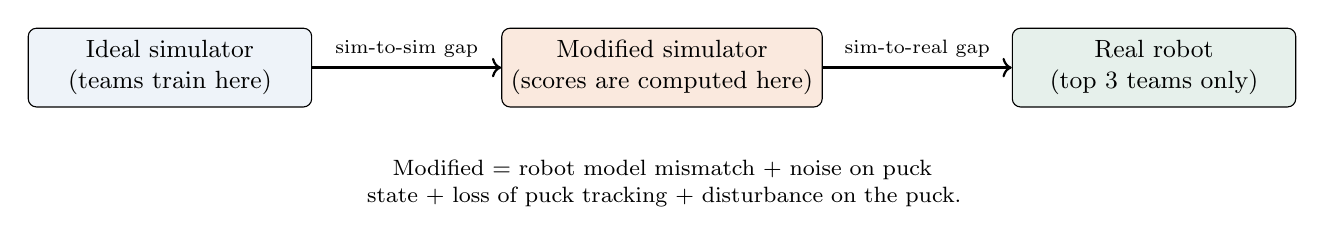
\begin{tikzpicture}[node distance=1.2cm, every node/.style={font=\small},
 box/.style={draw, rounded corners=3pt, minimum width=3.6cm, minimum height=1.0cm, align=center, fill=cblue!8},
 mod/.style={draw, rounded corners=3pt, minimum width=3.6cm, minimum height=1.0cm, align=center, fill=corange!15}]
\node[box] (ideal) {Ideal simulator\\(teams train here)};
\node[mod, right=2.4cm of ideal] (mod) {Modified simulator\\(scores are computed here)};
\node[box, right=2.4cm of mod, fill=cgreen!12] (real) {Real robot\\(top 3 teams only)};
\draw[->, thick] (ideal) -- node[above]{\scriptsize sim-to-sim gap} (mod);
\draw[->, thick] (mod) -- node[above]{\scriptsize sim-to-real gap} (real);
\node[below=0.55cm of mod, text width=9.5cm, align=center, font=\footnotesize]
 {Modified = robot model mismatch + noise on puck state + loss of puck tracking + disturbance on the puck.};
\end{tikzpicture}
\caption{The three worlds of the challenge (paper, Sec.~2).}
\end{figure}

\begin{idea}[One sentence to remember]
\emph{When a system is trained in a clean simulator and scored in a messier one, the messy
factors are not equally harmful: measurement \textbf{noise} is the one that the usual filters
already fix, while \textbf{losing the object} and \textbf{unmodelled forces on it} are the ones
that break the system.}
\end{idea}

% ============================================================ 3
\section{Glossary}

\begin{center}
\begin{tabularx}{\textwidth}{@{}l X@{}}
\toprule
Term & Meaning \\
\midrule
Puck & The air hockey disc. Slides on an air cushion, so it has very little friction. \\
Mallet & The paddle held by the robot, used to hit the puck. \\
Optitrack & A motion-capture system: several infrared cameras track reflective markers and give a very accurate 3D position at high rate. It is not a normal camera image pipeline. \\
Observation noise & Random error added to the measured puck position and velocity. \\
Tracking loss & The tracker stops following the puck for a while. \\
Disturbance & An outside influence on the puck that the simulator model does not include. Here it stands for the airflow of the table. \\
Model mismatch & The robot in the evaluation simulator has different masses, friction, damping and controller gains than the one the teams trained on. \\
Ablation study & Switch factors on or off one at a time to see how much each one changes the result. \\
Sim-to-sim gap & Difference between two simulators. Here: training simulator versus evaluation simulator. \\
Deployability score (DS) & A penalty count for violating safety limits. Not about ball estimation, so we skip it. \\
Inductive bias & Prior knowledge built into a method (physics, kinematics, geometry) instead of learned from data. \\
State observer / filter & A program that turns noisy measurements into a better estimate of the true state, e.g.\ a Kalman filter. \\
EKF & Extended Kalman filter. A Kalman filter that linearises a nonlinear model at each step. \\
MPC & Model predictive control. Plan a short future trajectory with a model, apply the first part, repeat. \\
RL, PPO, SAC, DreamerV3 & Reinforcement-learning methods used by several teams. Not needed for our chapter. \\
Episode & One run of a task from start to end. Here up to 500 control steps (10 s at 50 Hz). \\
\bottomrule
\end{tabularx}
\end{center}

% ============================================================ 4
\section{The paper, section by section}

\subsection{Introduction: five identified problems (paper, Sec.~1)}
The authors argue that machine-learning benchmarks are often too clean to reflect real robots,
and list five issues the challenge is built around:
\begin{enumerate}
\item \textbf{Safety}: the robot must not damage itself or the environment.
\item \textbf{Imperfect models}: it is hard to model a real system; learning methods must cope
with mismatch.
\item \textbf{Limited data}: real data are expensive, so the sim-to-real gap must be bridged with
little real data.
\item \textbf{Reactiveness}: dynamic environments need real-time decisions, often without a GPU.
\item \textbf{Observation noise and disturbances}: they ``will inevitably exist'' and
must be handled.
\end{enumerate}
For us only the fifth point, and partly the fourth (CPU only, which we also chose), is directly
relevant.

\subsection{The setup (paper, Sec.~2 and Appendix A.1)}
\begin{itemize}
\item Two Kuka LBR iiwa~14 arms and an air hockey table, plus a MuJoCo model of the same.
\item \textbf{Simulation frequency 1000~Hz, control frequency 50~Hz} (Table~1, paper).
\item The \textbf{observation} contains the puck position $[x,y]$, yaw angle $\theta$ and
\textbf{velocity} $[\dot x,\dot y,\dot\theta]$, plus the robot joint positions and velocities
\textbf{(paper)}. Notice that the environment hands the agent a puck \emph{velocity}, not only a
position. In their evaluation this velocity is also noisy, and teams had to filter it.
\item The control command is a desired joint position or velocity.
\end{itemize}

\subsection{The three tasks, the stages and the metrics (paper, Sec.~2.1--2.2)}
\textbf{Qualifying stage} has three sub-tasks: \emph{Hit} (shoot the puck into the goal),
\emph{Defend} (stop an incoming puck) and \emph{Prepare} (move the puck to a good position
without losing it). Each is scored by a success rate, and the overall score is the mean of the
three. Each task was evaluated on \textbf{1000 episodes} \textbf{(paper)}. \textbf{Tournament
stage}: teams play full 15-minute matches. \textbf{Real-world stage}: the top three teams'
agents play on the real robots. The final ranking was based only on the simulated tasks.

The \emph{deployability score} counts penalties for violating end-effector, joint position and
velocity limits and for slow computation (more than $0.02$~s per step). It decides whether a team
is classed as deployable, improvable or non-deployable. This is about robot safety, not ball
estimation, so I only mention it so you know what the ``Penalty Points'' column in the tables
means.

\subsection{Results of the qualifying stage (paper, Sec.~3.1, Table~3)}
Success rates (paper):

\begin{center}
\small
\begin{tabular}{@{}lrrrr@{}}
\toprule
Team & Hit & Defend & Prepare & Score \\
\midrule
AiRLIHockey (winner) & 54.9\% & 84.5\% & 90.3\% & 73.8 \\
Air-HocKIT & 52.2\% & 79.0\% & 68.6\% & 66.2 \\
GXU-LIPE & 30.1\% & 29.5\% & 66.2\% & 37.1 \\
SpaceR & 14.4\% & 47.8\% & 47.8\% & 34.4 \\
Baseline (organisers) & 12.8\% & 25.4\% & 66.3\% & 28.5 \\
\bottomrule
\end{tabular}
\end{center}
The winner mostly used \textbf{imitation learning of an optimal-control policy} (paper, App.~A.6),
and the second team used plain reinforcement learning. The authors conclude that teams with
robotics experience and \emph{physical priors} did better than pure machine-learning teams.

\subsection{The ablation: which sim-to-sim factor hurts most? (paper, Sec.~3.1, Fig.~4)}
\label{sec:ablation}
This is the part we use most. The evaluation was repeated in \textbf{six} environments:
\begin{enumerate}
\item \textbf{Ideal}: no factor.
\item \textbf{Model mismatch}: only the robot-arm model differs.
\item \textbf{Observation noise}: only additive noise on puck position and velocity.
\item \textbf{Disturbance}: only an extra force on the puck (airflow).
\item \textbf{Tracking lost}: only random loss of puck tracking.
\item \textbf{All factors}: everything together (the real evaluation).
\end{enumerate}
\textbf{What the authors conclude (paper):} model mismatch plays a marginal role because the
closed-loop controller corrects it; observation noise has limited impact because most teams
applied a state observer that filters the noisy observation; \textbf{tracking loss and
disturbances ``majorly affect the outcome''}; the Hit task is the most sensitive, ``likely due to
the fast movements and sensitivity to small angular errors''; with all factors on, agents on
average do worse.

The paper prints no table for this figure. Reading the ``Average'' group of bars by eye:

\begin{center}
\small
\begin{tabular}{@{}lcccccc@{}}
\toprule
Task (average over teams) & Ideal & Mismatch & Obs.\ noise & Disturbance & Track lost & All \\
\midrule
Hit & 0.45 & 0.44 & 0.43 & 0.41 & 0.40 & 0.34 \\
Defend & 0.69 & 0.69 & 0.67 & 0.61 & 0.57 & 0.48 \\
Prepare & 0.69 & 0.67 & 0.66 & 0.64 & 0.63 & 0.55 \\
\bottomrule
\end{tabular}
\end{center}
\textbf{(read from chart, about $\pm0.02$)}. In words: for Defend, noise costs about 2 points,
disturbance about 8, tracking loss about 12, and all together about 21. The single-factor drops
add up to roughly the combined drop (here $0+2+8+12=22$ against $21$), so the factors look
roughly additive in these averages.

\begin{warn}[Read the ablation with a statistician's eyes]
\textbf{(1)} The difference between two success rates is only meaningful if it is larger than the
statistical noise. With $n=1000$ episodes and a success rate near $0.5$, one rate has a standard
error of $\sqrt{0.5\cdot0.5/1000}=1.6$ points, so its 95\% interval is about $\pm3.1$ points; the
\emph{difference} of two independent rates has about $\pm4.4$ points. So a 2-point ``noise'' effect
is \emph{inside} the noise, while a 12-point tracking-loss effect clearly is not. The authors
admit themselves that some improvements under single factors ``would probably disappear with more
task repetitions'' (paper, Sec.~3.1). \textbf{(2)} The per-team bars sometimes show a factor
\emph{improving} the result (e.g.\ disturbance for SpaceR on Hit), which again points to noise.
\textbf{(3)} Observation noise looks harmless \emph{only because the teams filtered it}. That is a
statement about ``noise plus a good filter'', not about noise itself. If a team had used raw
measurements, the answer could differ. For our chapter, where the filters are the \emph{thing
being compared}, we cannot reuse the conclusion; we must measure it.
\end{warn}

\subsection{Tournament and real robot (paper, Sec.~3.2--3.3)}
The winner of the tournament was again AiRLIHockey (33 points; SpaceR 21; Air-HocKIT 20), mostly
because of fast and accurate hits. On the real robot, the top three teams' agents were deployed
with an extra safety layer, and all of them played complete games. \textbf{Performance on the real
robot was ``considerably worse'' than in simulation, and it needed hand-tuning and
engineering}, so the outcome of the competition relied only on simulation (paper, Sec.~2.1).

\subsection{The $40$~ms delay (paper, Sec.~3.3)}
\label{sec:delay}
The key sentence is: ``Contrary to the simulation, real-world deployment is not a synchronous
process, and the system is affected by delays. The delays, approximately 40~ms, arise from
gathering the observation, action computation, and execution.''

\begin{warn}[What the 40 ms is, and what it is not]
(1)~It is a \textbf{one-sentence remark} about the real system. It is \textbf{not} part of the
ablation, and the modified simulator did \textbf{not} contain it. So the paper gives no
measurement of how much a delay hurts.
(2)~It is the delay of the \emph{whole loop}: observation gathering \emph{plus} computing the
action \emph{plus} executing it. It is not a camera latency and certainly not a depth-camera
latency.
(3)~The tracker was motion capture, not a camera.
So $40$~ms is a reasonable order of magnitude for ``total latency of a fast robot loop'', and
I would use it as a \textbf{placeholder} for the sensor delay in our simulation, labelled as such,
and then \textbf{vary it} (for example $0$, $20$, $40$, $80$~ms) instead of treating it as a fact.
I earlier wrote it in my notes as ``delay modelled from the Liu retrospective''; this is the
correct, weaker reading.
\end{warn}

\begin{toy}[Toy example: what does 40 ms mean for our ball?]
The camera image is stale by $40$~ms when the estimator sees it. A ball at speed $v$ has moved
$v\cdot0.04$ since the picture was taken:
\begin{center}
\small
\begin{tabular}{@{}rrr@{}}
\toprule
ball speed & distance moved in 40 ms & in pixels (3 m, 60\textdegree, 7.2 mm/px) \\
\midrule
0.5 m/s & 2.0 cm & 2.8 px \\
1 m/s & 4.0 cm & 5.5 px \\
3 m/s & 12.0 cm & 16.6 px \\
5 m/s & 20.0 cm & 27.7 px \\
\bottomrule
\end{tabular}
\end{center}
If the estimator knows the delay and the ball keeps sliding, it can \emph{predict forward} by
$40$~ms. With friction deceleration $\mu=0.5$~m/s$^2$ a constant-velocity forward prediction is off
by only $\tfrac12\mu t^2 = 0.4$~mm. \textbf{But a wall bounce inside the window breaks this.} If
the ball bounced somewhere in the last $40$~ms ($E=0.8$, $v=3$~m/s), the straight-line forward
prediction is wrong by up to $(1+E)\,v\,t = 0.22$~m, and by $0.11$~m on average. A ball at $3$~m/s
in our $2$~m arena hits a wall about $2$ times per second (average of my own estimate
$0.66\,v$ hits per second), so about $7.6\%$ of the $40$~ms windows contain a bounce. That is why
delay and bounces must be studied \emph{together} in our chapter.
\end{toy}

\subsection{How the top solutions handled the puck (paper, Sec.~3.4 and Appendix A.6--A.9)}
\label{sec:solutions}

\paragraph{AiRLIHockey (winner), App.~A.6.1: state estimation and prediction.}
The puck dynamics are modelled as \textbf{piecewise (locally) linear with three modes}:
(a)~sliding freely, (b)~in contact with the wall, (c)~in contact with the mallet. In each mode~$i$
the next puck state is Gaussian:
\[
\Pr\nolimits_i\!\left(s^p_{k+1}\mid s^p_k,s^m_k\right)=\mathcal N\!\left(A_i s^p_k+B_i s^m_k,\ \Sigma_i\right),
\]
where $s^p=(x^p,\dot x^p)$ is the puck state, $s^m$ the mallet state, $A_i,B_i$ are matrices
\textbf{learned from simulation data}, and $\Sigma_i$ is a learned process-noise covariance for
each mode. Because the mode switches are discontinuous (contacts), they cannot simply multiply
Gaussians through, so an \textbf{extended Kalman filter} estimates the puck state over time for a
given mallet state. This is the idea of paper 01 (Jankowski et al.), which we will read in detail
later; here it is a one-paragraph summary. Note: \emph{learning is used for the state estimation and
prediction}, as in our chapter's plan.

\paragraph{Air-HocKIT, App.~A.8.3: noise handling.}
The observation noise in evaluation is ``additive noise on the puck positions and velocities and
loss of puck tracking'', where \textbf{loss of tracking means the observed puck position stays
constant and hence the observed velocity is zero}. This situation never happens in training, which
makes it a ``major change for the agent''. Their fix: (i)~put the noise and tracking loss
\emph{into} the training simulator; (ii)~model the additive noise as a Gaussian whose parameters
are fitted by maximum likelihood from observed and smoothed puck trajectories; (iii)~apply a
\textbf{Kalman filter} to the observations; (iv)~give the agent both the observed and the
estimated position, ``in case tracking of the puck is lost''; (v)~compute the velocity by
\textbf{finite differences of the estimated position}.

\paragraph{RL3\_polimi, App.~A.9.4.}
Training included both noise and tracking loss; they approximated the noise model; they used the
\textbf{simplified Kalman filter that the organisers provide in the challenge code}; and they
found their rule-based policies were \emph{more sensitive to the noisy observations than to the
loss of tracking}, the opposite of the average result.

\subsection{Key problems, limitations and conclusion (paper, Sec.~3.5--4)}
The teams named two main research problems: satisfying constraints, and decisions at different
time scales (for AiRLIHockey, fast control needs \emph{long-horizon prediction}). The paper's own
limitations are important for us:
\begin{itemize}
\item ``We assume a good perception system: we track the puck using the Optitrack motion capture
system. This assumption neglects \ldots perception.''
\item The conclusions ``suffer from a limited sample size''.
\item The real-robot stage was small and needed tuning.
\item ``Our sim-to-sim approach closely predicts the results we can expect on real-world
deployment'' (paper, Sec.~3.6).
\end{itemize}
The conclusion is that \textbf{physics priors and classical methods still beat pure data-driven
ones}, and that the future lies in combining both. This matches the plan of our chapter
(gray-box models first, learned estimators second).

% ============================================================ 5
\section{Numbers worth remembering}

\begin{center}
\small
\begin{tabularx}{\textwidth}{@{}X l@{}}
\toprule
Item & Value \\
\midrule
Simulation / control frequency & 1000~Hz / 50~Hz \textbf{(paper)} \\
Episode length & up to 500 steps = 10~s \textbf{(paper)} \\
Episodes per sub-task in the qualifying stage & 1000 \textbf{(paper)} \\
Real-system delay & ``approximately 40~ms'', whole loop \textbf{(paper)} \\
Tracking-loss model in the evaluator & observed position frozen, observed velocity $=0$ \textbf{(paper)} \\
Noise standard deviation, loss probability, loss duration & \textbf{not given} in the paper \\
Win rates in Table~3 & see Sec.~4.4 \textbf{(paper)} \\
Ablation averages & Sec.~4.5 \textbf{(read from chart, about)} \\
\bottomrule
\end{tabularx}
\end{center}

% ============================================================ 6
\section{Critical reading (my comments)}

\begin{warn}[1. Motion capture is not a depth camera]
Optitrack gives a clean, high-rate position of a marker. A depth camera, such as the one in our
simulator, adds depth noise that grows with distance, a small ball that covers few pixels, an
ambiguity between surface and centre, and occlusion by the robot. Conclusions about ``noise'' in
this paper should not be transferred to our noise.
\end{warn}

\begin{warn}[2. Silent tracking loss is a design choice, not a law]
In this evaluator, the tracker keeps reporting a value (the old position) and a velocity of zero,
\emph{without flagging that the data are stale}. The agent must discover it itself. A real
camera pipeline usually \emph{knows} when detection failed, so it can flag ``no measurement''.
The two cases are very different for a filter: a flagged gap can be skipped (predict only),
while a silent stale value looks like a valid measurement that says ``the ball stopped'' and can
\emph{drag the estimate to a halt}. We need to decide which one we model, or both.
\end{warn}

\begin{toy}[Toy example: silent hold versus flagged gap]
Ball at $3$~m/s, $\mu=0.5$~m/s$^2$, the tracker is lost for $0.2$~s. The true ball moves
$3\cdot0.2-\tfrac12\cdot0.5\cdot0.2^2=0.59$~m. A raw (silent, held) measurement is wrong by
$0.59$~m at the end of the gap and reports speed $0$. A filter that \emph{knows} the gap and just
predicts with constant velocity is wrong by only $\tfrac12\mu t^2=1$~cm, if no wall is hit. For a
$0.5$~s gap the numbers are $1.44$~m (silent) against $6.3$~cm (flagged).
\end{toy}

\begin{warn}[3. The ``sim-to-sim predicts sim-to-real'' claim]
The paper says sim-to-sim ``closely predicts'' real-world results, but also says that performance
on the real robot was ``considerably worse'' than in simulation, and it gives no quantity that
compares the two (for instance a rank correlation). It is a hope, not a result. This is the
SRCC idea from the paper 10 guide.
\end{warn}

\begin{warn}[4. Single-factor ablation hides interactions]
Switching on one factor at a time, then all, tells us about the sum but not about
\emph{interactions}. The chart averages look additive, but with only these six conditions we
could never see a pair like ``tracking loss \emph{and} delay'' that is much worse than their
sum. In our chapter delay and bounces clearly interact (previous toy), so a full grid is
better than the one-at-a-time design.
\end{warn}

\begin{warn}[5. The ablation is about task success, not about estimation error]
All numbers are success rates of the whole agent. They mix control, planning and estimation.
For our chapter, where the contribution is the estimator comparison, we should measure
estimation and prediction error directly, and use success rate only at the end.
\end{warn}

% ============================================================ 7
\section{What this means for our chapter}

\begin{ours}[Take-away 1: copy the ablation design, and improve it]
Our conditions on the \emph{same} launches (same seeds): \textbf{ideal}, \textbf{noise only},
\textbf{dropout only}, \textbf{delay only}, \textbf{all}, and later pairs (delay $\times$ dropout,
noise $\times$ delay). Report for each: prediction error at several horizons and the number of
launches, with confidence intervals; use a \emph{paired} comparison because the launches are the
same. Our dataset has $500$ launches (50 speeds $\times$ 10), a bit smaller than $1000$; we can
add more because it costs only compute.
\end{ours}

\begin{ours}[Take-away 2: tracking loss has two versions in our camera]
In \texttt{sensing/camera.py}, \texttt{detect} already returns \texttt{None} when the ball is not
seen. That is a \textbf{flagged} loss. The Liu evaluator's \textbf{silent} loss (freeze the last
position, velocity zero) is an additional, harsher scenario. I propose to implement the loss as a
setting: \texttt{flagged} (default for the main comparison, because a camera pipeline knows when
detection failed) and \texttt{silent\_hold} (a robustness test, copying the paper). This is a
\textbf{decision for you}.
\end{ours}

\begin{ours}[Take-away 3: delay as a swept parameter]
Use $40$~ms as the default placeholder, labelled ``from Liu et al., total loop delay, not a
camera latency'', and sweep it. At $60$~Hz a frame lasts $16.7$~ms, so $40$~ms is $2.4$ frames.
Delay should be modelled in the sensor stage (the estimator receives a measurement stamped $t$ at
time $t+\text{delay}$), and the estimator must know the stamp to compensate.
\end{ours}

\begin{ours}[Take-away 4: baselines taken from the participants]
Two baselines are directly implementable and need no neural network: (a)~\textbf{Kalman filter on
position, velocity by finite differences of the filtered position} (Air-HocKIT), and
(b)~\textbf{piecewise-linear modes with an EKF} (AiRLIHockey, paper~01). Our Step~3 baselines
should include both, plus a plain finite-difference one, as the lower bound.
\end{ours}

\begin{ours}[Take-away 5: the metric]
The paper's success-rate-only evaluation is not enough for an estimator comparison. We use
\textbf{position and velocity error now}, \textbf{prediction error at $0.2$, $0.5$, $1.0$~s}, and
\textbf{catch success} at the very end.
\end{ours}

\begin{eqbox}[What we still need from other papers]
Depth-noise model (paper 12), what makes a small tracked ball hard (paper 18), the EKF with
friction and collisions (paper 19) and the piecewise-linear filter (paper 01). This paper is
the \emph{design guide} for the sensor-imperfection experiment, not the source of its numbers.
\end{eqbox}

% ============================================================ 8
\section{Test yourself}

\begin{enumerate}
\item What are the six environments of the ablation, and what did the authors conclude about
observation noise versus tracking loss? Why does that conclusion depend on the teams using filters?
\item The winning team was not the one with the most advanced learning. What did it use learning
for?
\item In the paper's evaluator, what happens to the observed puck position and velocity when the
tracking is lost?
\item What is the difference between a flagged and a silent tracking loss, and which is more
dangerous for a Kalman filter? Why?
\item A ball moves at $4$~m/s and the measurement is $40$~ms old. How far has it moved? How many
pixels is that at $7.2$~mm/pixel?
\item The paper says the real-world delay was ``approximately $40$~ms''. Name two reasons why this
is not the same as the latency of a depth camera.
\item With $n=1000$ episodes and a success rate of $0.7$, what is the 95\% interval of one rate,
and of the difference of two independent rates? (Answer: about $\pm2.8$ and $\pm4.0$ points.)
\item Why does the single-factor ablation design miss interactions, and how would you test for
them?
\item Which parts of this paper are \emph{not} usable for a depth-camera chapter, and why?
\end{enumerate}

\appendix
\section{Map of the paper}
\begin{center}
\small
\begin{tabularx}{\textwidth}{@{}l X@{}}
\toprule
Paper part & Content and where it is in this guide \\
\midrule
Sec.~1 & Five issues: safety, imperfect models, limited data, reactiveness, noise (Sec.~4.1) \\
Sec.~2 & Setup, stages, metrics (Sec.~4.2--4.3) \\
Sec.~3.1 & Qualifying results and the \textbf{ablation} (Sec.~4.4--4.5) \\
Sec.~3.2--3.3 & Tournament, real robot, \textbf{40~ms} (Sec.~4.6--4.7) \\
Sec.~3.4 & Participants' solutions (Sec.~4.8) \\
Sec.~3.5--3.6, 4 & Key problems, \textbf{limitations}, conclusion (Sec.~4.9) \\
App.~A.1 & Simulated environment details (Sec.~4.2) \\
App.~A.5 & Real-world deployment and safety layer (not needed) \\
App.~A.6.1 & AiRLIHockey state estimation: piecewise linear modes + EKF (Sec.~4.8) \\
App.~A.8.3 & Air-HocKIT noise handling (Sec.~4.8) \\
App.~A.9.4 & RL3\_polimi noise filtering (Sec.~4.8) \\
\bottomrule
\end{tabularx}
\end{center}

\end{document}
